\documentclass[main.tex]{subfiles}

\begin{document}

\section{Issue 2554}
\label{sec:2554}

When trying to change the zoom value by clicking the zoom button, the zoom label on the right lower corner updates correctly, but when trying to zoom in using the key shortcut (CTRL + '+'/'-') or via the view menu, the zoom label doesn't update.

\subsection{Steps}
\label{subsec:steps2554}

\begin{enumerate}[noitemsep]
\item Launch Boostnote
\item Click on the zoom button on the right lower corner
\item Change the zoom level
\item Verify that zoom label was successfully altered
\item Change the zoom level using the key shortcut (CTRL + '+'/'-') or the view menu
\item Verify that zoom label was unsuccessfully altered
\end{enumerate}

\textbf{Result:} The key shortcut doesn't work

\clearpage

\subsection{Requirements}

The key shortcuts for \textit{zoom in}, \textit{zoom out} should modify the zoom label on the right lower corner, however, the key shortcuts just zoom in and zoom out, and don't alter it.\\

\begin{figure}[htbp]
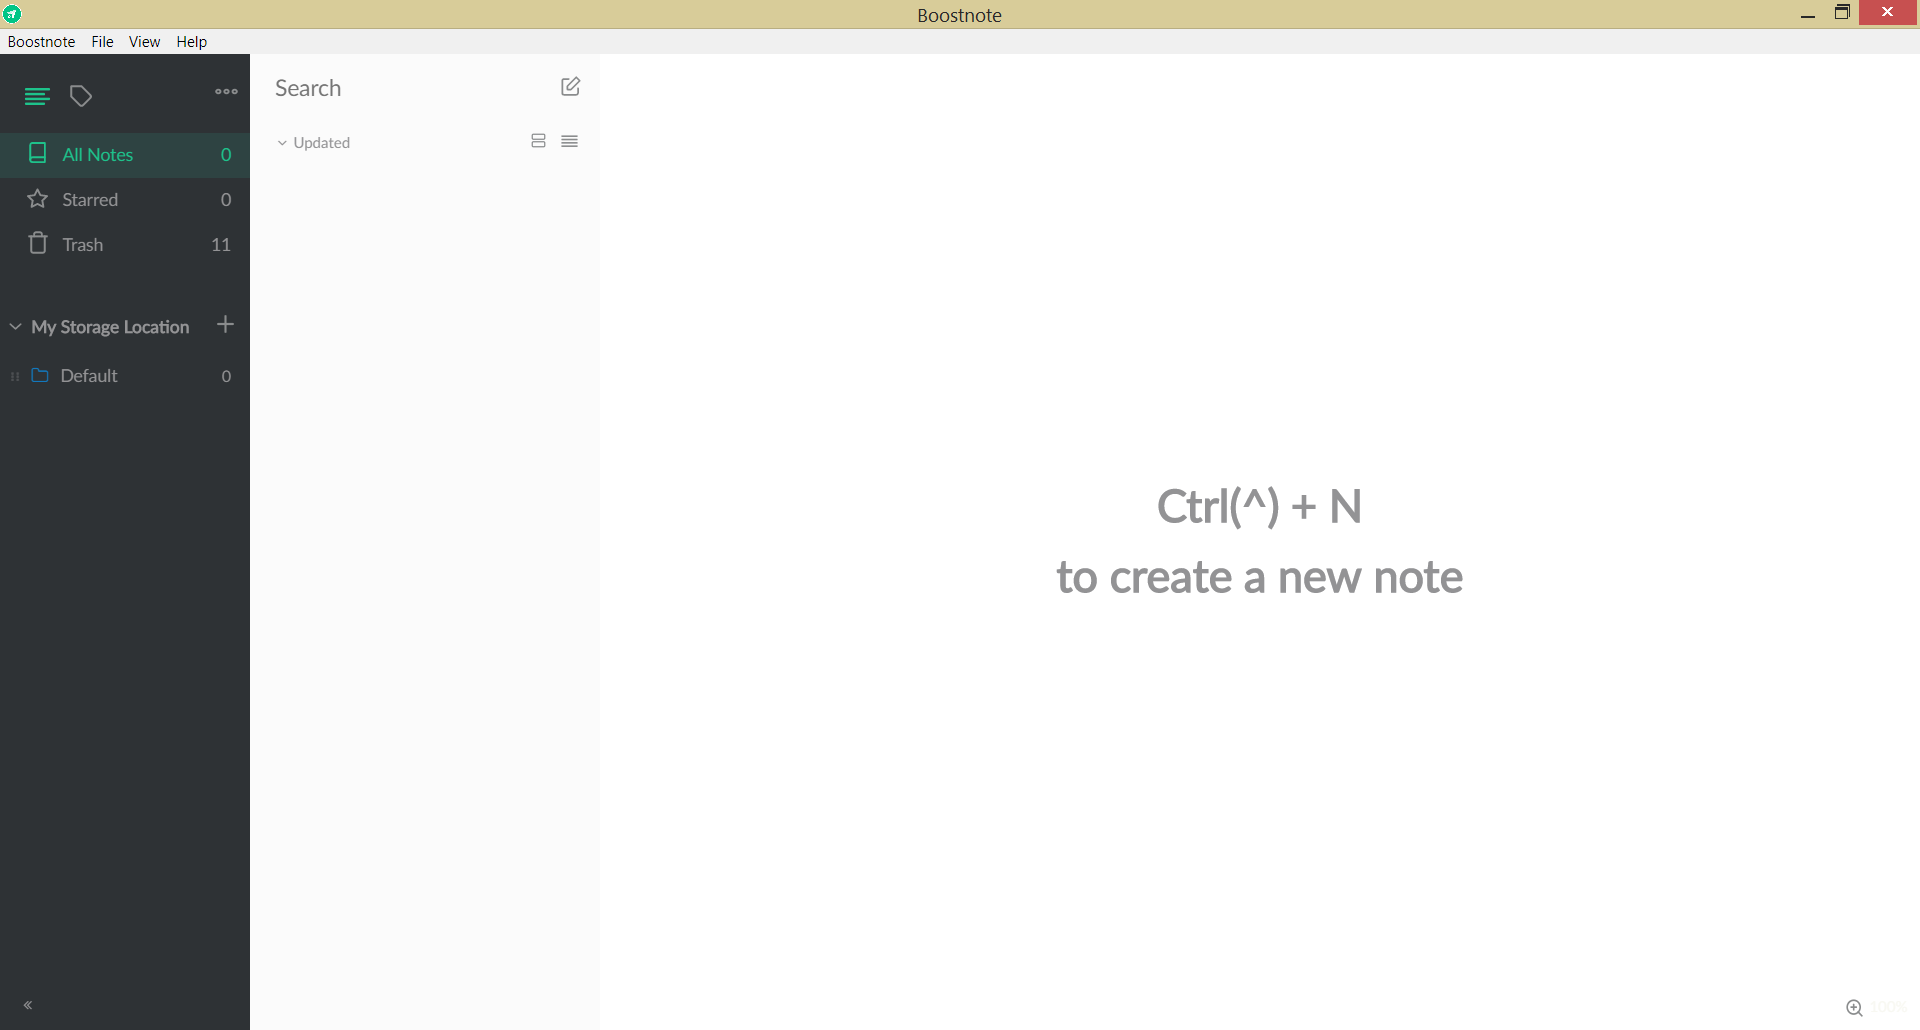
\includegraphics[scale=0.2]{images/normalZoom.png}
\centering
\caption{Normal Zoom}
\label{fig:normalzoom}
\end{figure}

\begin{figure}[h]
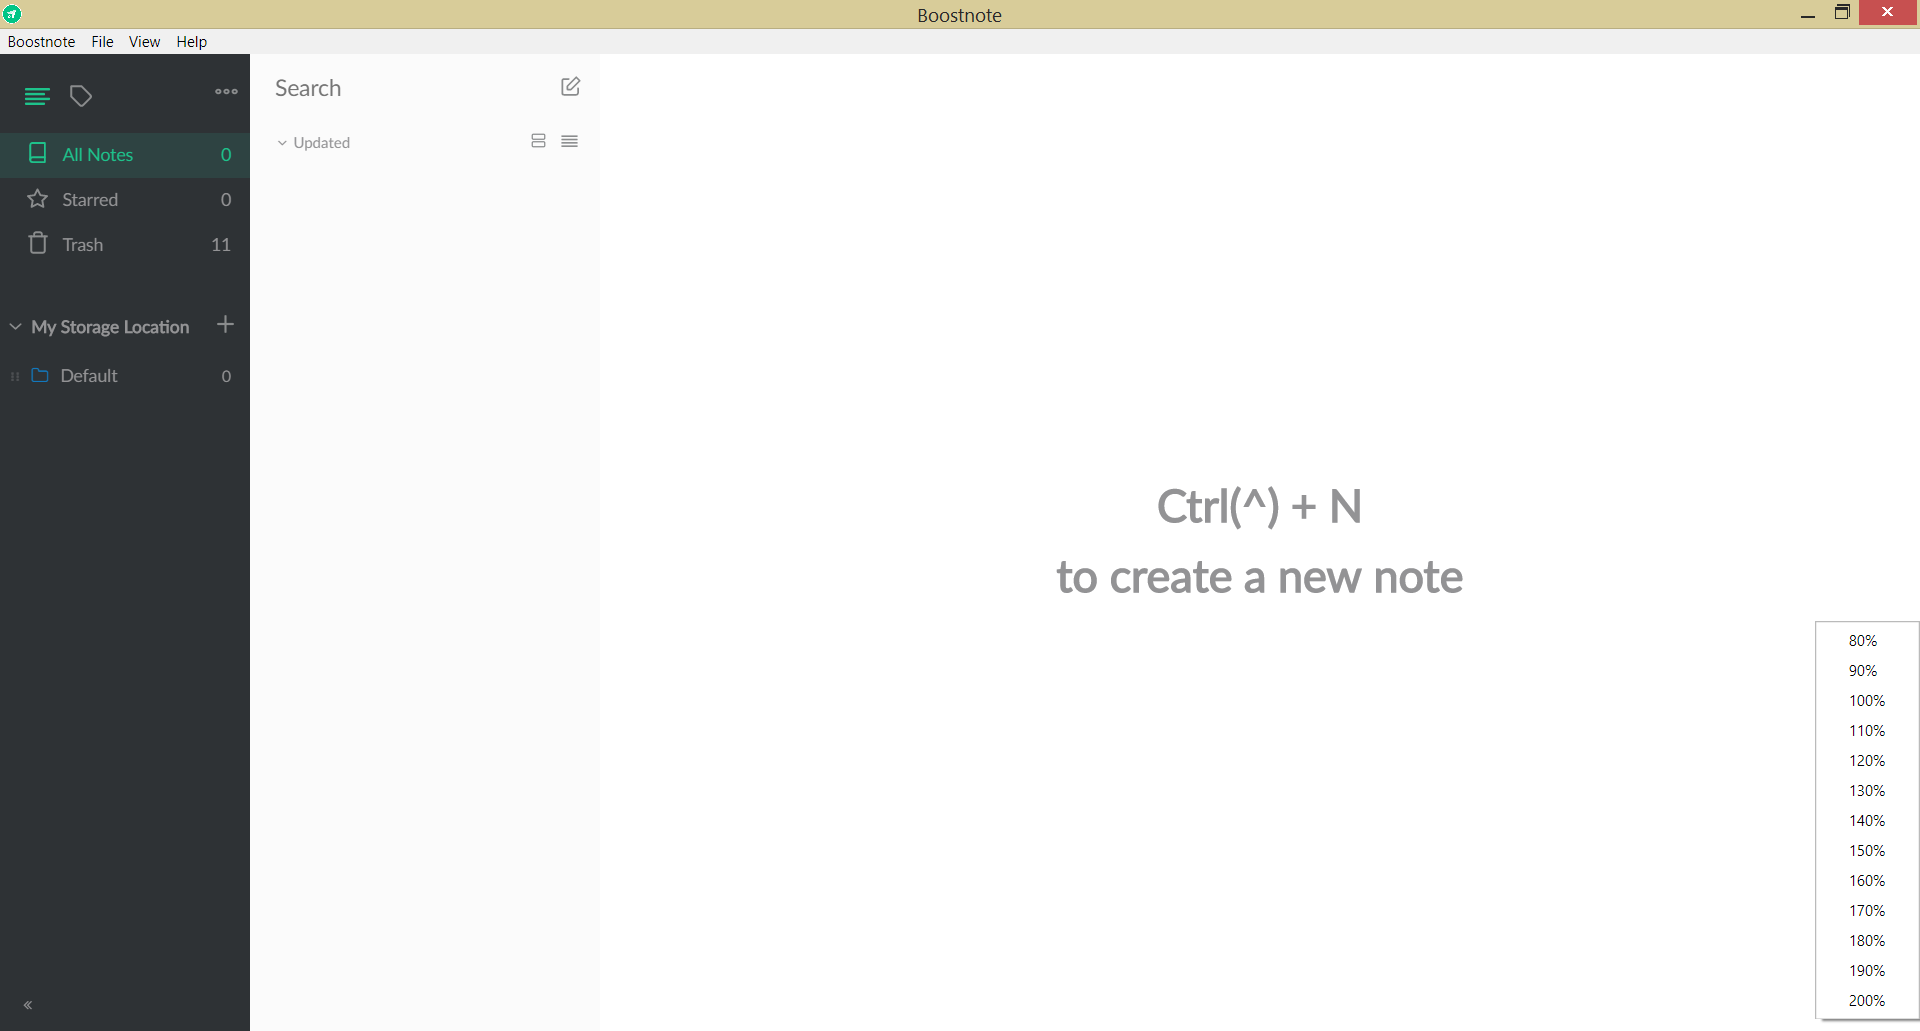
\includegraphics[scale=0.2]{images/zoomMenu.png}
\centering
\caption{Zoom Menu}
\label{fig:zoommenu}
\end{figure}

\begin{figure}[h]
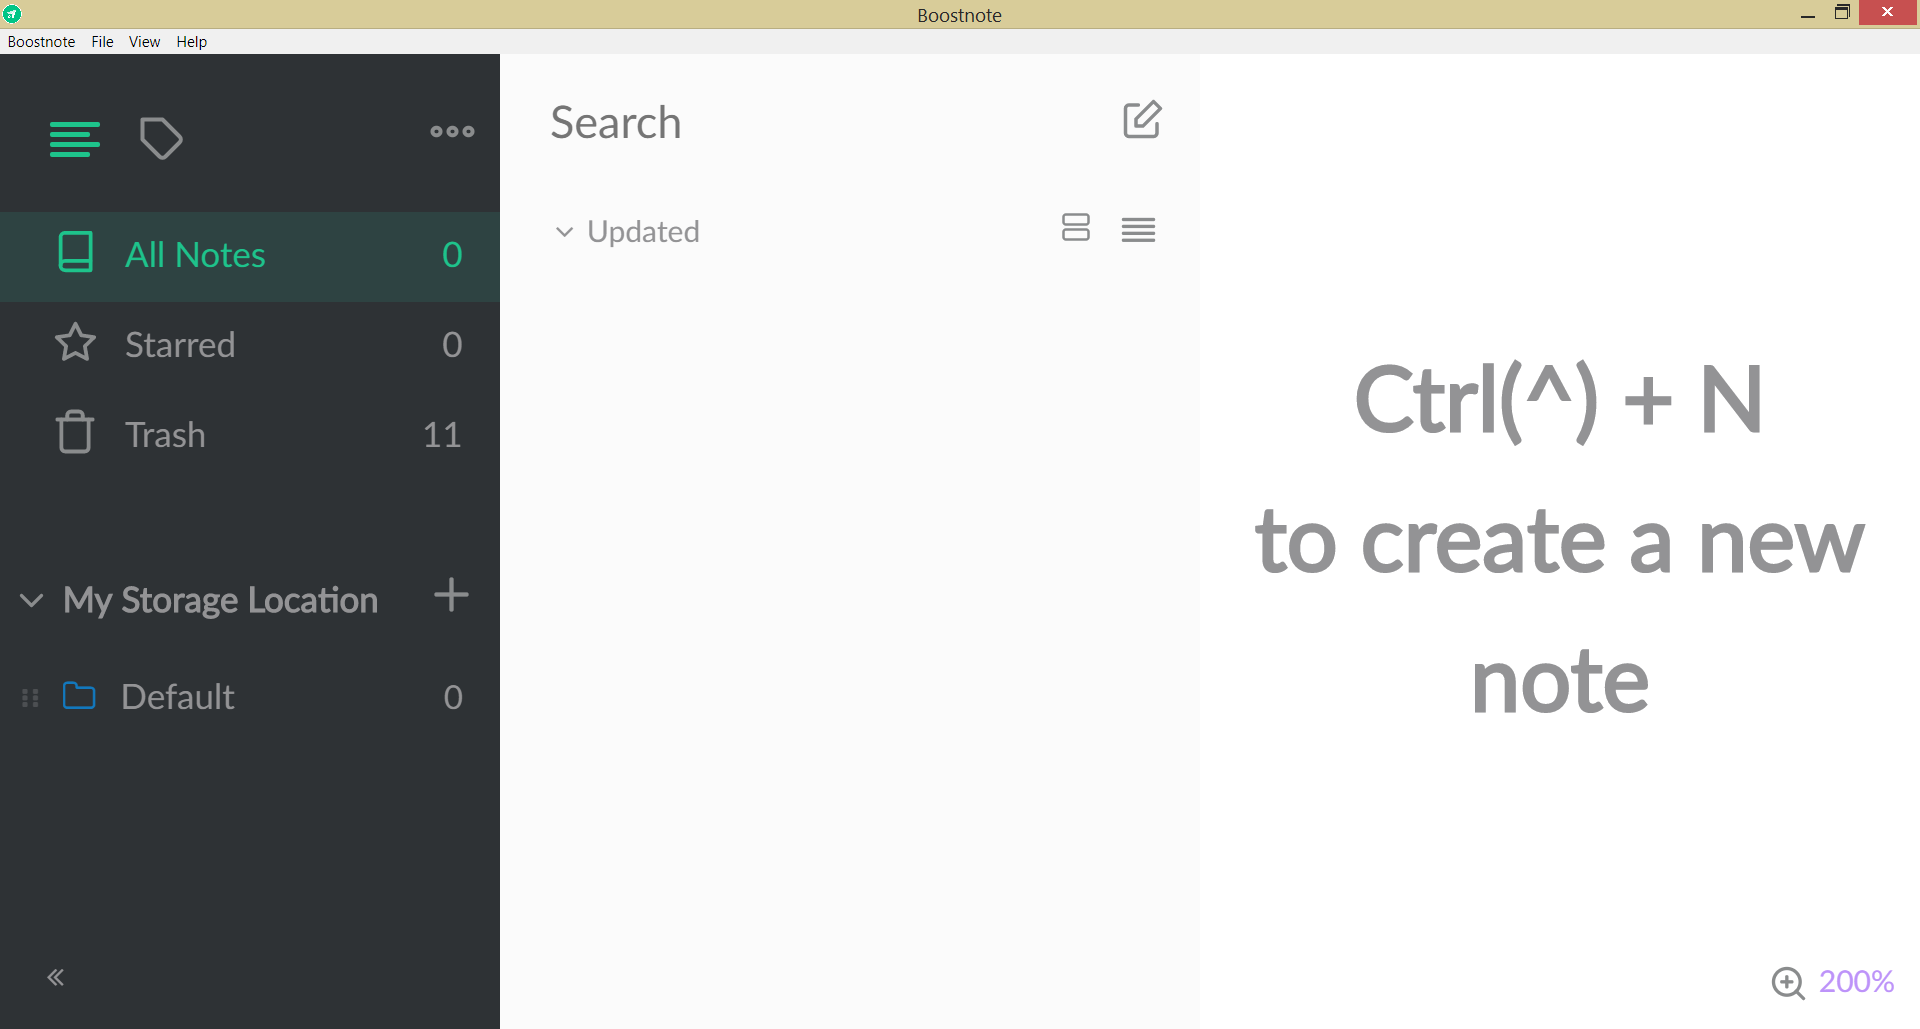
\includegraphics[scale=0.2]{images/zoomIn.png}
\centering
\caption{Zoom level at 200\% and label update}
\label{fig:zoomupdated} % bad label
\end{figure}

\begin{figure}[h]
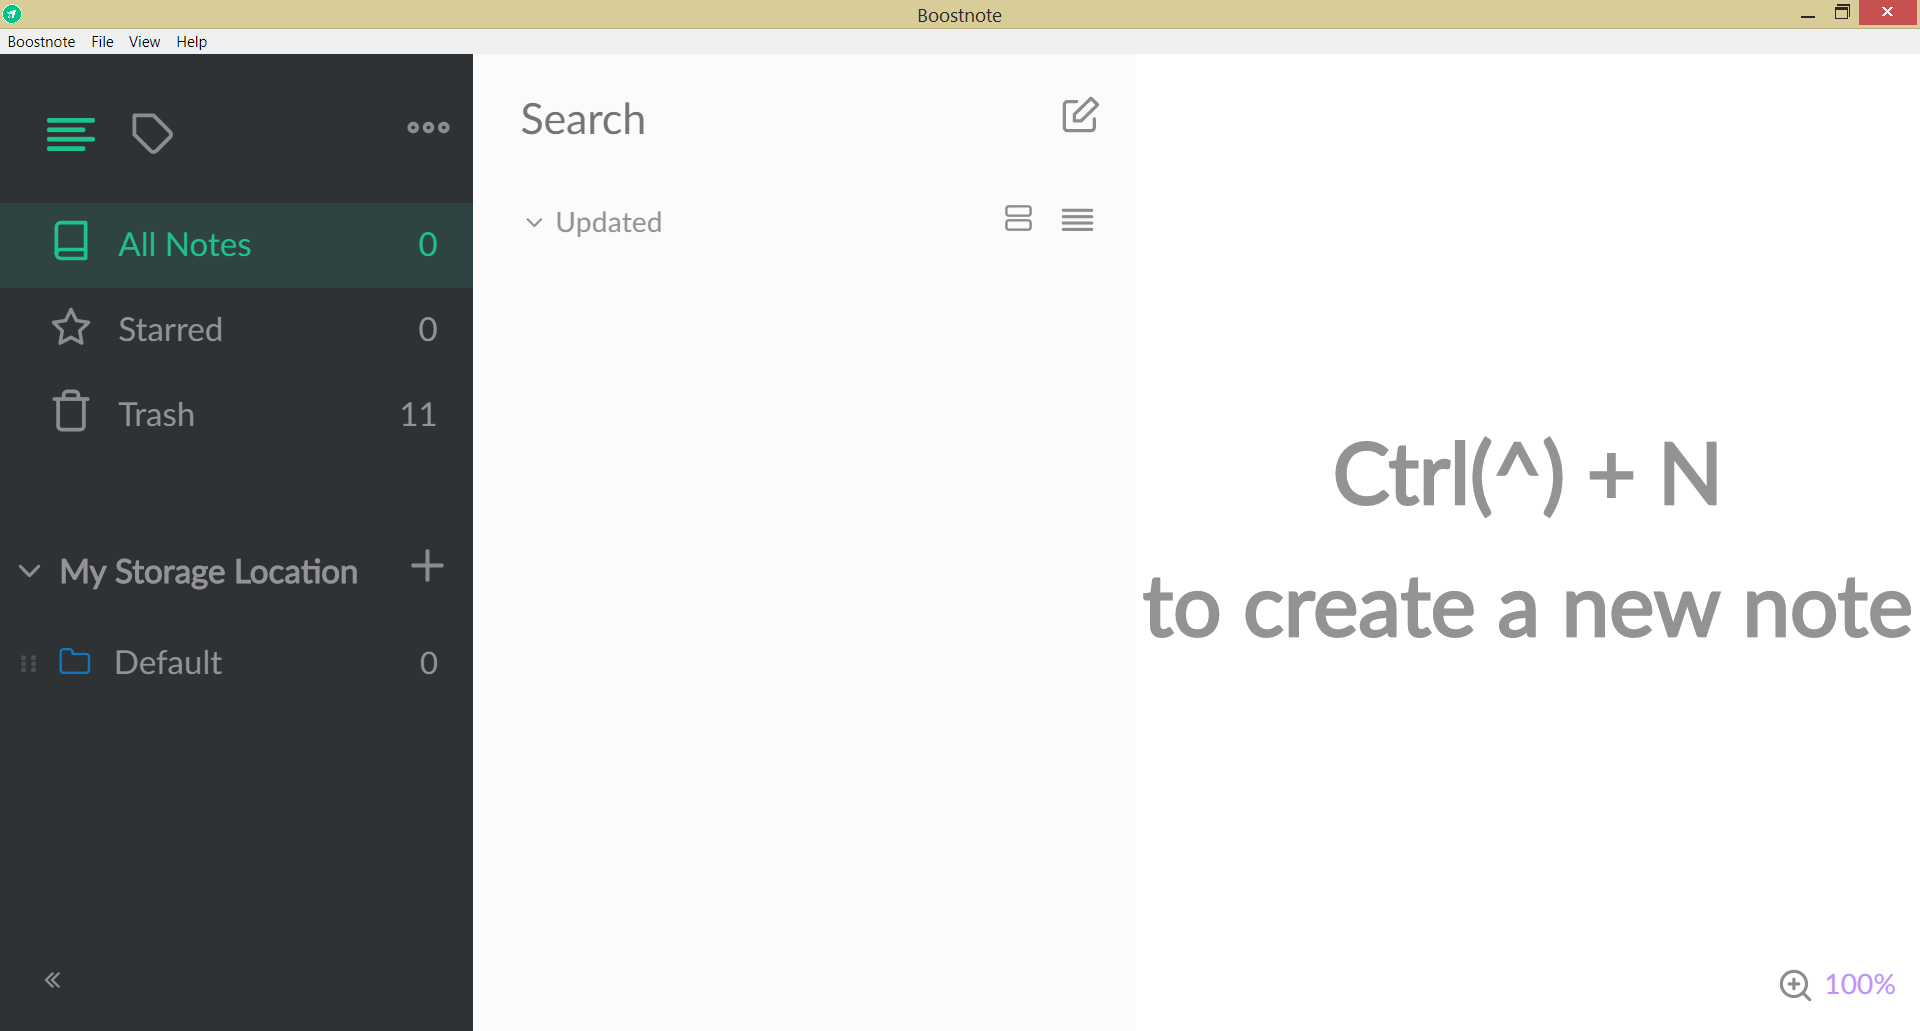
\includegraphics[scale=0.2]{images/zoomInUn.png}
\centering
\caption{Zoom level increased with key shortcut and label not updated}
\label{fig:zoomnotupdated} % bad label
\end{figure}
\clearpage

In \textbf{main-menu.js}, the Menu template (Electron) is created and there, the 'Zoom In' and 'Zoom Out' options are added to the view menu.

The menu itens are roles (labels with pre-made listeners) for the zoom in and zoom out buttons as electron has specific listeners for these actions:

\begin{itemize}
\item \textbf{zoomIn} - Zoom in the focused page by 10\%.
\item \textbf{zoomOut} - Zoom out the focused page by 10\%. 
\end{itemize}

CTRL+ is associated to Zoom In and CTRL- is to Zoom Out by association as triggers to modify the zoom.\\

The problem is that, when you zoom in or out using the views menu, the browser window zoomfactor is altered, but the config isn't altered, only the browser window class. The browser window class is where the zoom is actually set and the config is where the zoom value is kept for easy access.

When the zoom is changed via the status bar zoom (on the right bottom corner), not only is the browser window zoomFactor value changed, but also the config zoom value from which the current zoom label gets its value. The function used to do this is the \textbf{handleZoomMenuItemClick} function in \textbf{StatusBar/index.js} which uses the \textbf{setZoom} and inheretly the \textbf{saveZoom} function from\textbf{ ZoomManager.js}.\\

The label is defined in the render function of the StatusBar on StatusBar/index.js and as we can see, it get se zoom value from the config.
\clearpage

\subsection{Source Code Files}

\begin{figure}[htbp]
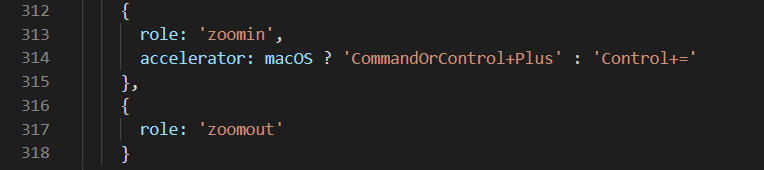
\includegraphics[scale=0.5]{images/mainMenu.png}
\centering
\caption{main-menu.js}
\label{fig:filemain-menu}
\end{figure}

\begin{figure}[htbp]
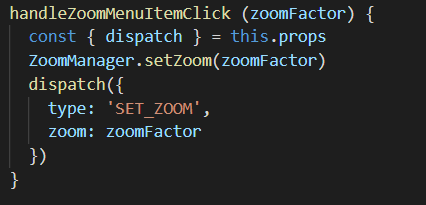
\includegraphics[scale=0.6]{images/handlerZoom.png}
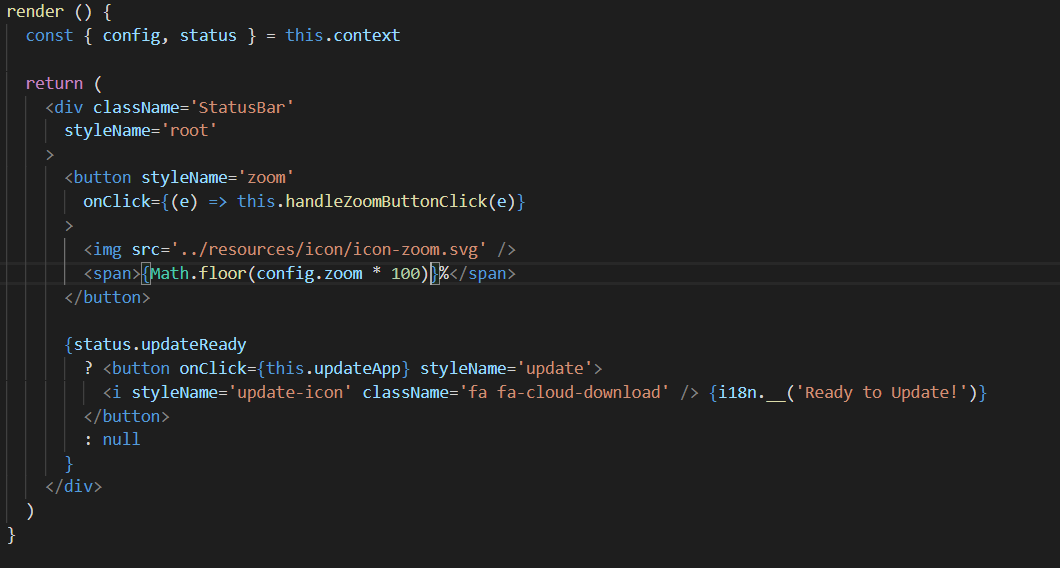
\includegraphics[scale=0.4]{images/render.png}
\centering
\caption{StatusBar/index.js}
\label{fig:statusbarindex}
\end{figure}

\begin{figure}[htbp]
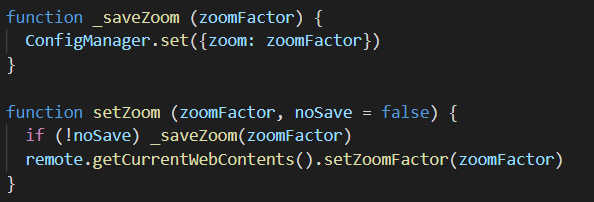
\includegraphics[scale=0.7]{images/zoomManager.png}
\centering
\caption{ZoomManager.js}
\label{fig:zoommanager}
\end{figure}

\begin{figure}[htbp]
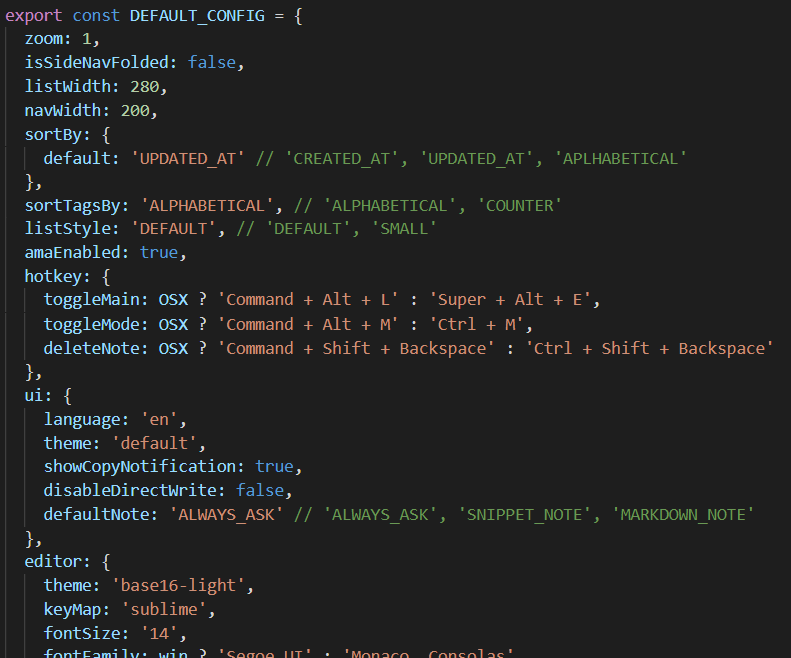
\includegraphics[scale=0.5]{images/export.png}
\centering
\caption{ConfigManager.js}
\label{fig:configmanager}
\end{figure}
\clearpage

\begin{figure}[htbp]
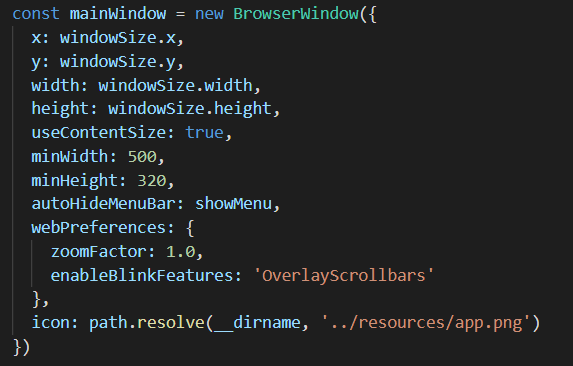
\includegraphics[scale=0.7]{images/mainWindow.png}
\centering
\caption{main-window.js}
\label{fig:main-window}
\end{figure}
\clearpage

\subsection{System Architecture}
\label{subsec:arch2554}

To better understand the system and how the modules interact, a diagram was created in which the different dependencies in boostnote can be observed. This type of diagram was picked because it gives an overview of the system without going into too much detail as the project is far too big. The most important dependency to this issue is the electron dependency as it is the framework used for the application.

\begin{figure}[h]
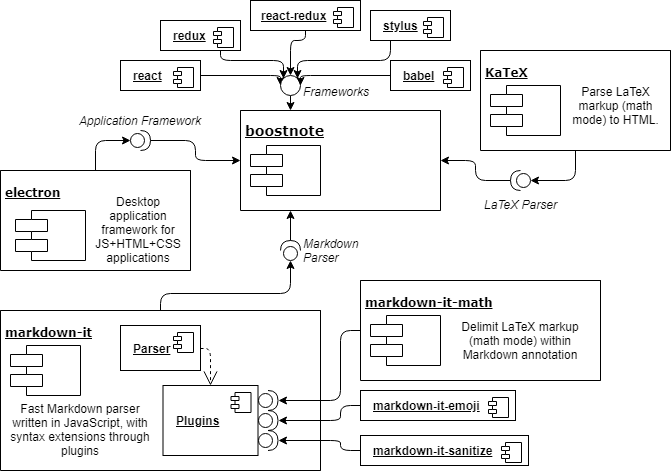
\includegraphics[scale=0.6]{images/diagram.png}
\centering
\caption{Boostnote's main dependencies}
\label{fig:boostnotearch}
\end{figure}
\clearpage

\subsection{Design of the fix}
\label{subsec:design2554}

The way to fix this issue is by either, getting the zoomFactor from the browser window instead of from the config or changing the menu item in the menu to not using the zoomin and zoomout role action, using instead another listener that also calls the config update.\\

In the following sequence diagram, it is explained how the zoomin/zoomout menu option click (which can be done with the hotkeys as well) will be handled. Boostnote will send a message to electron which will have a callback associated to it and will call the said function to handle it. The handler function will call handleZoomMenuItemClick function which is used by the zoom button to change the menu, it updates the zoom value on the config and on the browser window.\\

\begin{figure}[h]
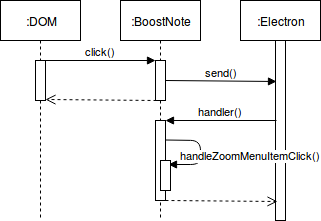
\includegraphics[scale=0.9]{images/dyagram-2554.png}
\centering
\end{figure}

\nocite{*}

\end{document}